%%%%%%%%%%%%%%%%%%%%%%%%%%%%%%%%%%%%%%%%%%%%%%%%%%%%%%%%%%%%%%%%%%%%%%
% How to use writeLaTeX: 
%
% You edit the source code here on the left, and the preview on the
% right shows you the result within a few seconds.
%
% Bookmark this page and share the URL with your co-authors. They can
% edit at the same time!
%
% You can upload figures, bibliographies, custom classes and
% styles using the files menu.
%
%%%%%%%%%%%%%%%%%%%%%%%%%%%%%%%%%%%%%%%%%%%%%%%%%%%%%%%%%%%%%%%%%%%%%%

\documentclass[12pt]{article}

\usepackage{sbc-template}

\usepackage{graphicx,url}

\usepackage[brazil]{babel}   
\usepackage[utf8]{inputenc}  
     
\sloppy

\title{Gestão Pessoal de Credenciais de Acesso a Serviços Digitais}

\author{Felipe Juris Jacques\inst{1}, Eduardo Dalcin\inst{1} }

\address{
  Especialização em Gestão de Tecnologia da Informação
  \\
  Instituto Federal de Educação, Ciência e Tecnologia Farroupilha Campus Panambi
  \\
  (IFFAR) -- Caixa Postal 98787 -- 740 -- Panambi -- RS -- Brazil
}

\begin{document} 

\maketitle

\begin{abstract}
  This meta-paper describes the style to be used in articles and short papers
  for SBC conferences. For papers in English, you should add just an abstract
  while for the papers in Portuguese, we also ask for an abstract in
  Portuguese (``resumo''). In both cases, abstracts should not have more than
  10 lines and must be in the first page of the paper.
\end{abstract}
     
\begin{resumo} 
  Este meta-artigo descreve o estilo a ser usado na confecção de artigos e
  resumos de artigos para publicação nos anais das conferências organizadas
  pela SBC. É solicitada a escrita de resumo e abstract apenas para os artigos
  escritos em português. Artigos em inglês deverão apresentar apenas abstract.
  Nos dois casos, o autor deve tomar cuidado para que o resumo (e o abstract)
  não ultrapassem 10 linhas cada, sendo que ambos devem estar na primeira
  página do artigo.
\end{resumo}


\section{Introdução}

All full papers and posters (short papers) submitted to some SBC conference,
including any supporting documents, should be written in English or in
Portuguese. The format paper should be A4 with single column, 3.5 cm for upper
margin, 2.5 cm for bottom margin and 3.0 cm for lateral margins, without
headers or footers. The main font must be Times, 12 point nominal size, with 6
points of space before each paragraph. Page numbers must be suppressed.

Full papers must respect the page limits defined by the conference.
Conferences that publish just abstracts ask for \textbf{one}-page texts.

\section{Credenciais de Acesso a Serviços Digitais} \label{sec:firstpage}

Qualquer serviço digital que exija autenticidade para identificar usuários
utiliza credenciais de acesso.
Embora cada serviço tenha credenciais únicas, eles compartilham padrões
comuns que os usuários conhecem.
Além disso, os serviços digitais têm contratos que os usuários devem aceitar,
mas a tecnologia por trás da segurança não é transparente para os usuários.
No entanto, é responsabilidade do usuário operar corretamente e respeitar
práticas de segurança comuns.

Ao se cadastrar, para possuir uma conta de usuário em um serviço digital,
é comum fornecer informações pessoais básica de identificação do usuário.
Esse cadastro dará origem a um conjunto de credenciais de acesso de uso
indiviual, que é utilizado para ter acesso ao respectivo serviço digital,
normalmente um identificador unico do usuário como telefone, CPF, nome ou
e-mail e uma senha que deve ser forte e segura, de conhecimento exclusivo
do usuário.

\subsection{Segurança de Serviços Digital}

Por mais sofisticados que os serviços digitais possam ser, não existe
garantias de segurança. É fundamental mitigar os riscos de segurança
por meio de práticas individuais.

As credenciais de acesso devem ser protegidas para evitar que terceiros
mal-intencionados as usem para obter vantagens indevidas.
Deixar credenciais vulneráveis pode expor o usuário a riscos ilimitados,
como roubo de informações, extorsão, invasão e mais.

Em um cadadstro de conta de usuário é importante fornecer apenas informações
necessárias e verdadeiras, informando apenas o mínimo necessário para
minimizar a exposição pessoal, considerando quem terá acesso a elas.

\section{Processo de Autenticação}

Quando um usuário acessa um serviço digital, ele faz isso por meio do
processo de autenticação (login), fornecendo duas informações: uma
identificação única (telefone, nome ou e-mail) e uma senha secreta.
É fundamental que a senha seja aleatória e não contenha informações
que possam ser facilmente memorizadas e principalmente, não deve conter
informações pessoais, pois isso pode ser descoberto por pessoas
mal-intencionadas.
Além disso, informações pessoais podem ser obtidas de várias maneiras,
como em perfis públicos do usuário.

\subsection{Multi Fator de Autenticação}

A autenticação multifator (MFA) é uma medida de segurança adicional que
exige dois ou mais fatores de verificação para acessar uma conta ou
recurso online.
Isso aumenta a dificuldade de acesso não autorizado, pois mesmo com a
senha, o atacante precisaria de fatores adicionais, como um código
enviado ao smartfone ou e-mail, uma impressão digital ou outro tipo de
verificação adicional.

A MFA se tornou uma prática padrão em serviços digitais, como bancos,
redes sociais e sistemas corporativos, fornecendo uma camada adicional
de segurança contra roubo de identidade e fraude cibernética.
Porém, não existe um padrão de MFA, cada serviço digital tem suas
próprias políticas de segurança.

\subsection{Duplo Fator de Autenticação}

O duplo fator de autenticação (2FA), autenticação em dois fatores (ADF) ou
até mesmo verificação em duas etapas (TFA) é uma medida de segurança
adicional que exige um segundo fator além da senha, como um código enviado
ao smartfone ou um dispositivo token (token de hardware).
Isso torna mais difícil para os atacantes acessarem contas online, mesmo
que eles obtenham a senha.

É possível usar diversos dispositivos simultâneos para armazenar as chaves
de duplo fator de autenticação e é indispensável realizar cópias de
segurança em nuvem ou arquivo digital.
No entanto, alguns serviços não oferecem o duplo fator de autenticação ou
exigem aplicativos proprietários, então é importante estar atento a
política de segurança e recursos de recuperação de acesso de contas.

Muitos serviços online oferecem o duplo fator de autenticação como opção
para aumentar a segurança dos usuários.
Ativar o duplo fator de autenticação é uma etapa importante para proteger
informações pessoais e é recomendável habilitá-lo sempre.

Um uso comun do duplo fator de autenticação é por meio do smartfone,
utilizando um aplicativo de autenticação de dois fatores para gerar
códigos de autenticação em tempo real sem conexão com a internet.
Embora cada serviço possua maneiras diferentes de ativar o duplo fator
de autenticação, normalmente é necessário acessar a configuração de
segurança da conta do usuário, procurar a opção de ativar o duplo fator
de autenticação ou algo relacionado ao termo.
Será apresendao um código QR para ser fotografado pelo aplicativo no
smartfone, em seguida será necessário digitar o código gerado pelo
aplicativo para ativar o duplo fator de autenticação.

Independente do aplicativo a ser usado para armazenar as chaves de
duplo fator de autenticação, é importante realizar cópias de segurança
em nuvem ou em arquivo digital para evitar perda de acesso às contas
de usuário.

\section{Phishing}

Phishing é um tipo de ataque cibernético onde criminosos tentam obter
vantagem ou obter informações confidenciais, como senhas, informações
pessoais e até detalhes de cartões de crédito, por meio de comunicações
fraudulentas.
Este termo deriva da palavra "fishing", que significa pescar em inglês,
aludindo à ideia de lançar iscas para capturar vítimas desavisadas.

Os ataques de phishing podem ocorrer através de e-mails, mensagens de
texto e chamadas telefônicas fraudulentas, serviços online falsos que
se assemelham muito com os verdadeiros, aplicativos malignos em lojas
de aplicativos, postagens e propagandas enganosas em redes sociais e
anúncios fraudulentos de internet, onde os golpistas se passam por
entidades legítimas para persuadir as pessoas a fornecerem suas informações
pessoais ou tirar vantagens para realizar ataques ao dispositivo.

A conscientização sobre esses golpes é crucial, pois o conhecimento é a
primeira linha de defesa contra os ataques cibernéticos.
É importante estar atento a mensagens suspeitas que solicitam dados
confidenciais ou contêm links e anexos desconhecidos. Para se proteger,
verifique a autenticidade das mensagens, não clique em links ou baixe
anexos de fontes desconhecidas e use soluções de segurança confiáveis.
Se receber um código de autenticação sem solicitar, não o informe a
ninguém e altere sua senha, pois pode ser uma tentativa de invasão.

\section{Multiplas Credencais de Acesso}

É comum que os usuários precisem gerenciar muitas credenciais de acesso
para diversos serviços online.
Nessa situação, não é recomendado repetir senhas para evitar que um invasor
descubra uma senha e acesse outros serviços.
É importante ter uma boa gestão de senhas e credenciais, incluindo a
possibilidade de recuperar senhas esquecidas.

\subsection{Lugares para Guardar Anotações de Credênciais}

É improvável que uma pessoa possa memorizar todas as credenciais de acesso,
então é necessário anotar as informações em algum lugar.
É importante anotar não só o login e senha, mas também outros detalhes,
como códigos de recuperação e descrições.

Ao usar um meio digital para anotações, é desejável usar um programa ou
aplicativos de confiança para proteger as informações. Além disso, é útil
evitar letras e caracteres semelhantes para evitar confusões.

\subsubsection{Anotações em Meio Físico}

É comum optar por anotar as informações das credenciais de acesso em um
caderno, já que requer menos desafios de informatização.
Deve se ter atenção a senhas, já que representar caracteres, letras
maiúsculas ou minúsculas pode ser mais difícil do que digitalmente e
causar confusões nos usuários mais despreparados.
Anotar em formato digital em um simples arquivo de texto envolve
complexidades, relacionados a necessidade de criptografia e cópias de
segurança para proteger os arquivos e evitar que possam ser
acessados por usuários indesejados ou invasores.

\subsubsection{Anotações em Serviços de Terceiros}

Os principais navegadores de internet oferecem recursos simples para
armazenar informações básicas das credenciais de acesso. Alguns até
com a possibilidade de sincronizar as informações entre dispositivos e
normalmente sem cobrar algum custo.

Por outro lado, para se ter mais controle de informações e recursos de
seguraça, existem programas e aplicativos de terceiros podem ser usados
para armazenar informações de credenciais de acesso, oferecendo diversas
vantagens. Normalmente essa opção exige algum tipo de assinatura.

De qualquer forma, deve-se evitar anotar senhas em no celular em
aplicativos de bloco de notas, aplicativos de mensagens em geral ou até
em formato de contatos de telefones, pois todos esses recursos não são
criptografados e normalmente são projatos para esses fins e podem ser
explorados usuários mal intencionados ou brechas de segurança.

\section{Trabalhos Relacionados}

Araujo et al. (2015), em seu artigo sobre a influência da Lei de Zipf na
escolha de senhas, analisa a criação de senhas seguras considerando a
teoria da informação e a lei de Zipf.
A lei de Zipf, que descreve a relação entre a frequência de ocorrência de
palavras e sua posição em uma lista ordenada, reduz a entropia das senhas
quando linguagens naturais são utilizadas, criando padrões que podem ser
explorados por atacantes.
A pesquisa conclui que a estratégia mais eficaz para criar senhas robustas
é a utilização de acrônimos, que aumenta a entropia por caractere em
aproximadamente 80%.
Outras estratégias, como o uso de palavras isoladas, passphrases e o
método Diceware, mostraram-se menos eficazes.
O estudo destaca a importância de escolher senhas que maximizem o espaço
de busca para ataques de força bruta, especialmente em sistemas com
restrições de comprimento.

Araujo et al. (2015), relata limitações de segurança em algum serviços
digitais na conclusão de seu artigo:
\begin{quote}
  Conforme observado em, 'Muitas vezes os sistemas restringem o comprimento da chave, por exemplo, a
  Microsoft restringe a 16 caracteres, muitas lojas de comércio eletrônico também restringem drasticamente o
  número de caracteres de uma senha. Lojas virtuais como Submarino e Americanas.com utilizam o máximo de 8
  caracteres, enquanto Netshoes utiliza 15 e, ainda, Mercado Livre, 20. Mais grave ainda são os bancos que,
  além de restringir o tamanho de sua senha, restringem também o alfabeto, aceitando apenas dígitos de 0 a 9.
  Essa prática de restringir o tamanho e tipo de caracteres nas senhas pode levar à criação de senhas mais
  fracas e, portanto, mais vulneráveis a ataques. \cite{araujo:2015}
\end{quote}

Berrios et al. (2023) destacam que o estudo em seu artigo "Factorizing 2FA:
Forensic analysis of two-factor authentication applications" analisou 15
aplicativos de autenticação de dois fatores (2FA) em diferentes sistemas
operacionais, incluindo Android, iOS e Windows 10, com foco na análise de
artefatos forenses deixados por esses aplicativos.
A pesquisa descobriu que a maioria dos aplicativos armazena informações em
texto simples ou criptografado/codificado, incluindo chaves secretas,
timestamps, nomes de contas e endereços de e-mail, o que pode permitir que
a funcionalidade 2FA seja contornada.
A descoberta de chaves secretas pode permitir que os examinadores forenses
gerem um OTP 2FA válido sem o uso do dispositivo original, reduzindo a
necessidade de manipular diretamente o dispositivo e potencialmente alterar
os dados.
O estudo destaca a importância da criptografia na proteção de dados do
usuário, especialmente em aplicativos 2FA, e sugere a análise de versões
futuras dos aplicativos e a exploração de outros tipos de autenticação
multifator.

Grimes (2019), em seu artigo "The many ways to hack 2FA" de argumenta que a
autenticação de dois fatores (2FA) não é infalível e pode ser facilmente
contornada.
A fraqueza central da 2FA reside no fato de que o token de acesso é
geralmente tratado da mesma forma, independentemente do formato ou tipo de
autenticação, o que significa que, uma vez obtido o token, o invasor pode
acessar o recurso protegido da mesma forma que o usuário legítimo.


Grimes (2019) descreve três métodos gerais para hackear a 2FA, incluindo
exploração de vulnerabilidades tecnológicas, ataques de engenharia social
e ataques físicos.
Além disso, são apresentados exemplos específicos de como a 2FA pode ser
comprometida, como roubo de cookies, sequestro de assunto, troca de SIM,
falsificação de SMS, geradores de código duplicados.
O autor conclui enfatizando a importância de discutir
as vulnerabilidades da 2FA para implementar e usar soluções mais seguras
e conscientizar administradores e usuários sobre os pontos fortes e fracos
da 2FA.

Para mais exemplos de como a 2FA pode ser hackeada, Grimes (2019) recomenda
o webinar ‘11 Ways to Defeat 2FA’, disponível em
https://info.knowbe4.com/webinar-11-ways-to-defeat-2fa (acesso em 04/11/2024).

\section{Metodologia}

A metodologia adotada é a pesquisa aplicada, que segundo Gil (2019), a
pesquisa aplicada, abrange estudos elaborados com a finalidade de resolver
problemas identificados no âmbito das sociedades em que os pesquisadores
vivem.

O público-alvo desta pesquisa são os usuários de serviços digitais,
especialmente aqueles que compartilham dados pessoais online e utilizam
plataformas digitais para fins, pessoais, profissionais ou até financeiros,
que, portanto, necessitam de maior atenção e cuidado com a segurança digital.

Este estudo utilizou uma abordagem quantitativa para investigar as práticas
de segurança digital dos usuários em relação às suas credenciais de acesso.
A coleta de dados foi realizada de forma anônima, através de um questionário
online elaborado na plataforma Microsoft Forms.
O questionário abordava temas como o uso de senhas, autenticação em dois
fatores, gestão de credenciais, entre outros, e foi divulgado em grupos de
WhatsApp.
A pesquisa garantiu a privacidade e confidencialidade das respostas,
assegurando o anonimato dos participantes.

Realizado uma avaliação prática dos aplicativos de autenticação de dois
fatores Google Authenticator, Microsoft Authenticator e Aegis em sistema
Android, durante um período um semestre. Os aplicativos foram selecionados
com base em sua popularidade e disponibilidade, bem como a presença de um
aplicativo de código aberto (Aegis) para fornecer uma perspectiva mais
diversificada.
Durante o período de teste, foram avaliados os recursos oferecidos por cada
aplicativo, incluindo a facilidade de uso, o gerenciamento de contas, os
recursos de segurança adicionais e a usabilidade geral.
Além disso, foram registrados os problemas e dificuldades encontrados
durante o uso diário dos aplicativos, a fim de avaliar sua eficácia e
eficiência em diferentes contextos.

Realizado uma busca para experimentar aplicativos para gerenciar
virtualmente as senhas de serviços digitais baseada do nos sistemas
operacionais Android e Windows.

\section{Resultados e Discussão}

\subsection{Pesquisa de Campo}

A pesquisa obteve uma amostra composta por 17 participantes, queresponderam
ao questionário voluntariamente durante um período de dois meses no segundo
semestre do ano de 2024.
35,3\% dos participantes trabalham na área de tecnologia a mais de 10 anos,
29\% na dos participantes estudam na área de tecnologia a mais de 10 anos,
e 76,5% dos participantes utilizam alguma tecnologia a mais de 10 anos.

Na pergunta sobre o uso de senhas fortes, 35\% dos participantes afirmaram
usar senhas muito grandes e aleatórias e 18\% utilizam frases longas
e criativas. Porém 29\% dos participantes utilizam senhas com base em uma
informação pessoal.

A respeito da memorização de senhas em navegadores, 59\% disseram digitar as
senhas uma única vez e permanecer logados.
Além disso, 41\% dos participantes utilizam sempre a autenticação em dois
fatores, sendo o Google Authenticator o mais usado.
A maioria dos participantes, 10, memoriza suas senhas, e 24\% já tiveram o
login roubado.
Por fim, a avaliação média dos participantes sobre a segurança dos serviços
digitais foi de 3,88, e sobre a segurança das suas próprias ações foi de
3,47.

Na pergunta aberta, 'Sinta-se livre para sugerir um aplicativo, software ou
serviço de segurança pessoal', houve apenas uma resposta.
O participante sugeriu: 'Joga fora Hotmail e Outlook e usa tudo da Google com
dados falsos (data de nascimento etc), aí ninguém consegue recuperar a conta,
a não ser você.
Visto que teus dados estão expostos em todos os lugares'.
Essa resposta possui preferencia clara aos serviços do Google em relação a
Microsoft e tem vies ao anônimato para fortalecer a segurança pessoal.

\subsection{Avaliação Prática dos Aplicativos de Duplo Fator de Autenticação}

Durante a avaliação prática dos aplicativos de duplo fator de autenticação,
foram identificados pontos positivos e negativos em relação à usabilidade,
segurança e eficácia dos aplicativos.

\subsubsection{Google Authenticator}

O Google Authenticator foi considerado o mais fácil de usar, com uma
interface simples, auto explicativa e intuitiva.
No entanto, o aplicativo não oferece recursos adicionais, cópias de segurança
é exclusivamente em nuvem e sómente é permitido instalar o aplicativo em um
aparelho GMS (Google Mobile Services).

Em um aparelho GMS, a memorização de senhas ou preenchimento automático de
senhas oferecida pelo Google não tem relação com esse aplicativo, na verdade
esse é um recurso do próprio aplicativo do Google.

\subsubsection{Microsoft Authenticator}\label{sec:figs}

Microsoft Authenticator, por sua vez, possui uma interface mais complexa com
poucas intruções de utilização do aplicativo.
Há recusros adicionais para as contas de usuários Microsoft, como a possibilidade de
inpecionar o historico de atividade e autenticar apenas confirmando a notificação
no smartfone, sem a necessidade de digitar o código do duplo fator de autenticação.
Há também diversos recursos diferentes, talvez o mais importante seja a possibilidade
de memorização de senhas ou preenchimento automático de senhas.

Cópias de segurança das chaves de duplo fator de autenticação é exclusivamente em
nuvem e somente é possível instalar o aplicativo em dispositivos GMS.
A Microsoft oferece recursos corporativos, então para quem utilizar esse
aplicativo para proteger sua conta corporativa, precisa usar uma conta pessoal
para realizar o cópias de segurança das chaves de duplo fator de autenticação, também
é possível utilizar outros aplicativos para essa finalidade, mas essa opção está um
pouco escondida.

Assim como o Microsoft Authenticator tem diversos recursos, há diversas instabilidades
relacioanado diretamente as contas de usuário Microsoft.
Em uma tentativa de instalar o aplicativo com uma conta de usuário que ainda não havia
duplo fator de autenticação, foi solicitado que a conta fosse verificada pelo proprio
aplicativo ainda não configurado, alternativamente era possível apenas digitar a senha,
tornando a experiência confusa.
Ainda na mesma tentativa, ao finalizar o processo de autenticação, houve um erro de
comunicação entre o aplicativo e o servidor, impossibilitando a utilização do aplicativo.

\begin{figure}[h!]
  \centering
  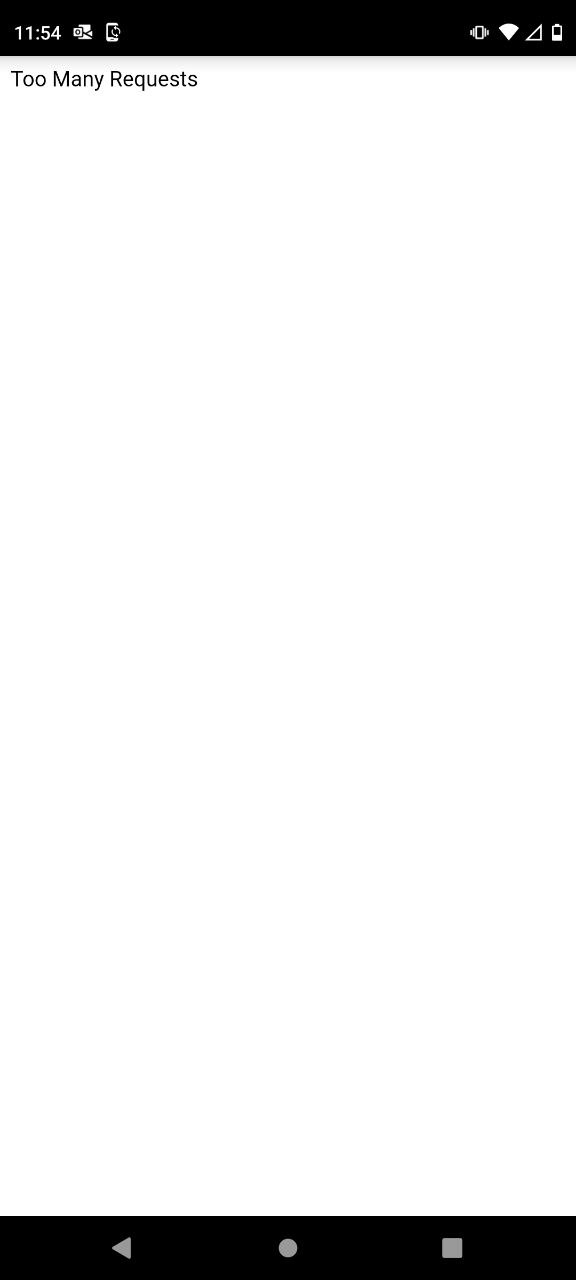
\includegraphics[width=0.3\textwidth]{./assets/microsoft_error_1.jpg}
  \caption{Erro de comunicação entre do aplicativo Microsoft Autenticator}
  \label{fig:MicrosoftAutenticatorErrorToManyReequests}
\end{figure}

Outro erro ocorreu ao tentar configurar uma outra conta de usuário que já utilizava o
duplo fator de autentiação para utilizar os recursos extras de autenticação, fucionando
de uma forma diferente, onde durante um processo de autenticação, será solicitado uma
confirmação de notificação no smartfone.
A aplicativo recebeu instruções para ativar o Bluetooth, embora atipico para esse tipo
de autentiação, ao tentar efetuar a autenticação, o aplicativo não respondeu e em tentativas
posteriores, ocorria erro no aplicativo.
No final, houve transtornos para recuperar o acesso a conta de usuário, pois nem mesmo os
metodos extras de autenticação funcionaram.

\begin{figure}[h!]
  \centering
  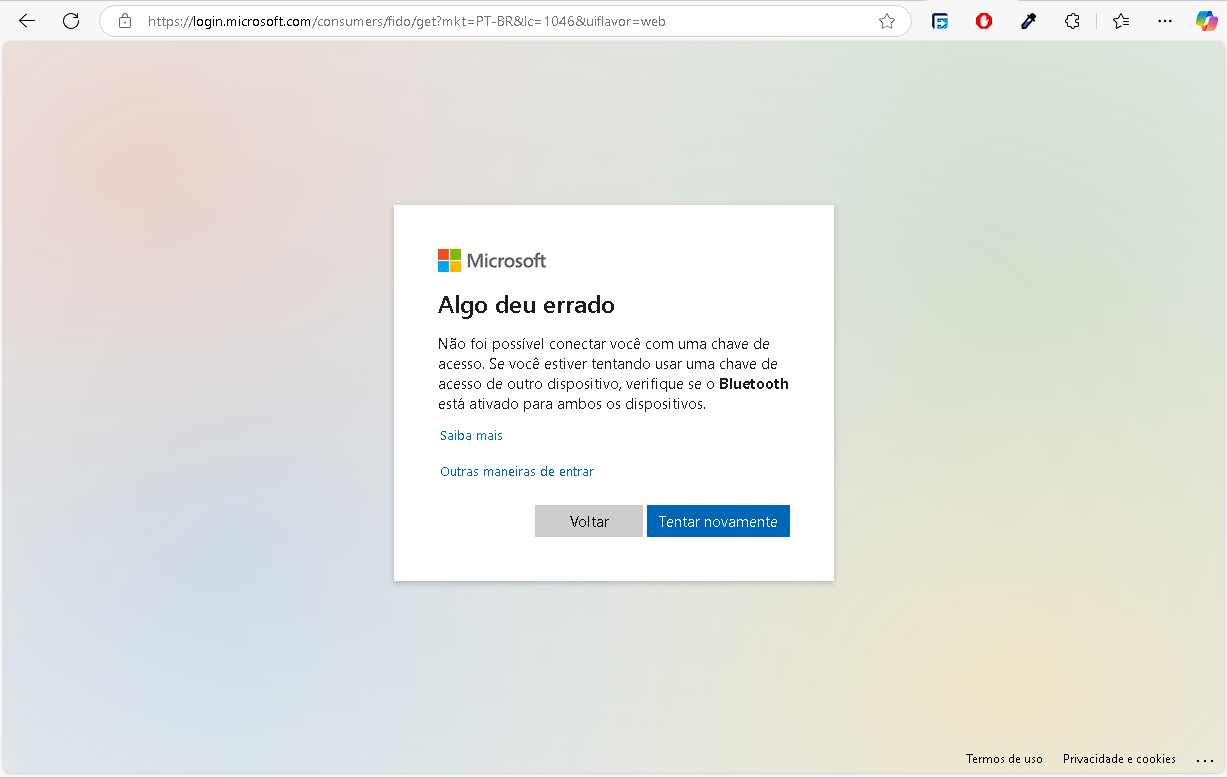
\includegraphics[width=0.7\textwidth]{./assets/microsoft_error_2.png}
  \caption{Erro no duplo fator de autentiação da Microsoft}
  \label{fig:Microsoft2FactoryAutenticatorError}
\end{figure}

\subsubsection{Aegis}

Já o Aegis, por ser um aplicativo de código aberto, oferece maior transparência
e controle sobre os dados do usuário, mas possui uma interface de configuração
e arquivos que pode ser menos amigável para usuários mais leigos.
Nele é possível adicionar e gerenciar chaves de autentiação de dois fatos,
exportar e importar cópias de segurançats para diversos aplicativos ou em formato de arquivos,
inclusive em formato criptografado.

A maior vantagem do Aegis é a possibilidade de instalar o aplicativo por meio da
loja de aplicativos de código aberto F-Droid, uma alternativa ao Google Play
Store, permitindo que o mesmo possa ser intalado em dispositivos Android sem GMS
ou AOSP (Android Open Source Project).

\subsection{Avaliação de Aplicativos de Gerenciamento de Senhas}

No sistema operacional Android com GMS o Google automaticamente oferece um popup
para salvar a senha no momento em que é digitada no processo de autenticação de
algum aplicativo ou serviço.
Como o Google não é especificamente um aplicativo de segurança, pode parecer um
pouco escondido a opção de gerenciar as senhas pelas configurações de conta.
Além do gerenciamento de senhas com sincronização em nuvem, é possível adicionar
anotações, exportar e importar em formato de plianilha CSV sem criptografia.

O mesmo pop-up do Android utilizado pelo Google pode ser substituido por
aplicativos de terceiros, como o Microsoft Authenticator, citado anteriormente
que oferece recursos adicionais para gerenciar senhas, sendo assim um aplicativo
praticamente completo para a segurança pessoal do usuário, com sincronização em
nuvem.
Também é possível adicionar anotações, exportar e importar em formato de
plianilha CSV sem criptografia.
O sistema operacional Windows não possui opção nativa ou pré instalada para
salvar senhas, as senhas gerenciadas por esse aplicativo são as mesmas salvas no
navegador de internet Microsoft Edge do Windows, que no Windows só funcionam
dentro do proprio navegador.

KeeWeb é um aplicativo de código aberto que oferece uma interface amigável para
gerenciar senhas, com maior foco no gerenciamento das anotações.
Diferente dos aplicativos citados anteriormente, o KeeWeb não é um aplicativo
nativo, mas sim um aplicativo web progressivo, que pode ser instalado em qualquer
dispositivo com navegador de internet, porém, sem integração com o sistema
operacional, ou seja, nele, o usuário vai apenas realizar anotações.
O KeeWeb permite salvar as anotações de senhas em formato de arquivos com ou sem
criptografia, os arquivos podem ser exportados localmente ou em nuvens de
serviços de terceiros em que o usuários tiver preferencia.

\section{Considerações Finais}

A pesquisa revelou que os participantes possuem um nível de conscientização sobre
a importância da segurança digital, demonstrado pelo uso de senhas fortes e pela
autenticação de dois fatores.
No entanto, algumas práticas de segurança, como senhas fracas e permanecer
autenticado, ainda podem ser melhoradas.

Uma parcela significativa dos participantes já teve problemas de segurança, o que
indica que as práticas atuais não são totalmente eficazes.
A pontuação média da segurança em serviços digitais e da segurança pessoal indica
espaço para melhorias das ações pessoais e dos serviços digitais.

A memorização de senhas em navegadores de internet pode expor o acesso ao serviço
sem exigir senha.
Embora a sincronia em nuvem seja suficientemente segura, não é solicitada uma
senha mestre para liberar a autenticação ou até para visualizar a senha.
Ambos os casos são escolhidas pelos usuários devido à conveniência sedutora de não
ter que se preocupar com senhas e pode permitir que quem tenha acesso ao
dispositivo acesse o serviço, o que é ainda mais inseguro se o dispositivo não
estiver protegido por um bloqueio de tela.

Felizmente, a autenticação em duas etapas é uma camada adicional de segurança que
pode proteger as contas dos usuários.
No entanto, essa tecnologia é práticamente restrita a dispositivos moveis.
Utilizar apenas um dispositivo, com cópias de segurança em nuvem e proteger o mesmo serviço de
nuvem nesse dispositivo pode ser uma armadilha que não é préviamente avisado aos
usuários.
Portanto, é importante possuir uma estrategia de recuperação do cópias de segurança ou possuir
mais de um dispositivo ao mesmo tempo para autenticação, escolhendo bem o
aplicativo e os dispositivos para essa situação, do contrário, em caso de perda
ou roubo do dispositivo, essa camada adicional de segurança pode dificultar o
acesso do proprio proprietário, principalmente se o usuário apenas utiliza o
smartfone.

Utilizar aplicativos de gerenciamento de senhas, apresentou grande praticidade,
especialmente para os serviços que não se mantem autenticados, solicitam a
autenticação com frequencia ou perdem a autenticação por defeito.
Porém os aplicativos de gerenciamento de senhas e navegadores de internet não
são perfeitos, em alguns casos, apresnetam o popup sob a caixa de entrada do
login, senha ou botões.
Já o KeeWeb, se não estiver configurado para o mesmo idioma do dispositivo, foi
prejudicado no sistema operacional Android, por ser um aplicativo web progressivo,
o Google Chrome insiste em traduzir o aplicativo e até mesmo as senhas, tornando
as senhas invalidas.

Todo o serviço que é bem feito, vai usar um algoritmo de derivação de chave e
nunca vai salvar a sua a senha de forma aberta.
Logo, se o mesmo limita o comprimento ou variabilidade de caracteres de sua senha,
é um grande indicativo de que o serviço não está preocupado com a segurança de
seus dados.

\bibliographystyle{sbc}
\bibliography{references}

\end{document}